Pentru folosirea sistemului, aplicația client trebuie instalată pe un dispozitiv ce rulează o versiune mai
mare sau egala cu 7.0 a sistemului de operare iOS. Aplicațiile server sunt deja instalate pe unul din 
serverele gazdei \textit{Heroku}, iar acestea nu necesită nici un fel de configurare. Odată instalată aplicația
client pe dispozitivul mobil, utilizatorul va putea să profite din plin de funcționalitățile sistemului. 

Rețeaua de socializare „GoodCitizen” este disponibilă la adresa \mbox{https://goodcitizen-a5f99.firebaseapp.com/}.
Aplicația web este instală pe unul dintre serverele gazdei \textit{Google Firebase}. Instalarea nu necesită 
nici o configurație în prealabil.

Web API-ul aplicației este instalat pe serverele din pachetele de servicii oferite gratis de Heroku.
Dacă nu este primește nici o cerere timp de 30 de minute, Web API-ul intră într-o starea de hibernare.
În momentul în care se primește o cerere, API-ul iese din starea de hibernare. Din acest motiv la o primă cerere după perioada de hibernare,
timpul de răspuns este mai mare. Web API-ul poate fi accesat la adresa \mbox{https://goodcitizen-api.herokuapp.com/}.
% \section{Testarea Web API-ului}
În procesul de dezvoltare a Web API-ului am folosit extensia browser-ului \textit{Google Chrome} numită \textit{Postman}.
Acesta este un client HTTP folositor în testarea serviciilor web expuse. Extensia este concepută
pentru a economisi timp, astfel ajută la creșterea productivității dezvoltatorilor.

\begin{figure}[h]
% 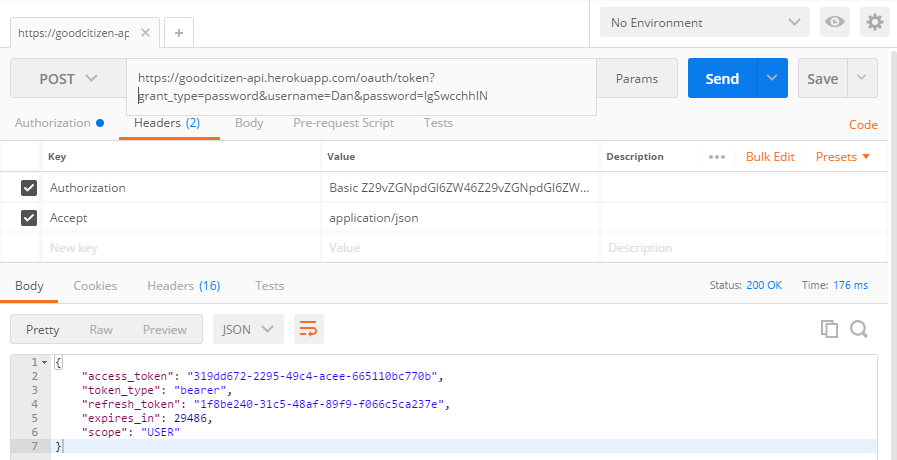
\includegraphics[height=0.45\linewidth]{postman.png}
 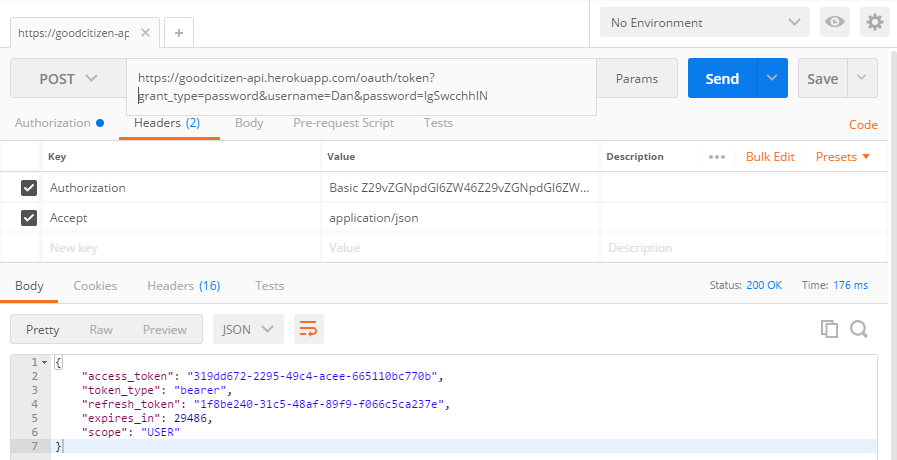
\includegraphics[width=\textwidth,height=\textheight,keepaspectratio]{postman.png}
\centering
\caption{Exemplu de cerere HTTP folosind Postman}
\label{fig:postman}
\end{figure}

În Figura.~\ref{fig:feedback} este reprezentată o cerere HTTP de tipul POST realizată cu \textit{PostMan}. 
Cerere are scopul de a obține token-ul folosit la autentificare în aplicație.
Totodată se poate observa și timpul de răspuns al cererii.

    Ca măsura de securitate am folosit HTTPS deoarece este recomandat ca token-urile de 
autentificare să fie trimise prin intermediul unei conexiuni criptate. Astfel sunt evitate 
atacuri cum ar fi MITM(\textit{Man in the Middle}).Într-un atac de tipul MITM, atacatorul 
se bazează pe interceptarea și alterarea comunicării dintre server și client. Astfel 
atacatorul poate obține token-ul de autentificare.
    Web API-ul folosește standardul CORS(\textit{Cross-origin resource sharing}). Acesta este un standard pentru 
a accesa resurse web de pe domenii diferite. Din motive de securitate browser-ele interzic cereri AJAX aflate în 
afara originii curente. CORS permite interacțiune intre scripturi web mult mai liber în afara 
domeniului original, astfel se realizează o integrare mai bună intre servicii web.
   



 